\documentclass{beamer} 
\usepackage[utf8]{inputenc}
 \usepackage{graphicx}
 
\title[About Beamer]
{Polyphase Filtering:  A Physicist's Understanding}
%Information to be included in the title page:
\author{Matthew B. Cooper}
\institute{New Jersey Institute of Technology}
\date{May 8th, 2019}
\begin{document}
 
\frame{\titlepage}
 
\begin{frame}
\frametitle{Introduction}
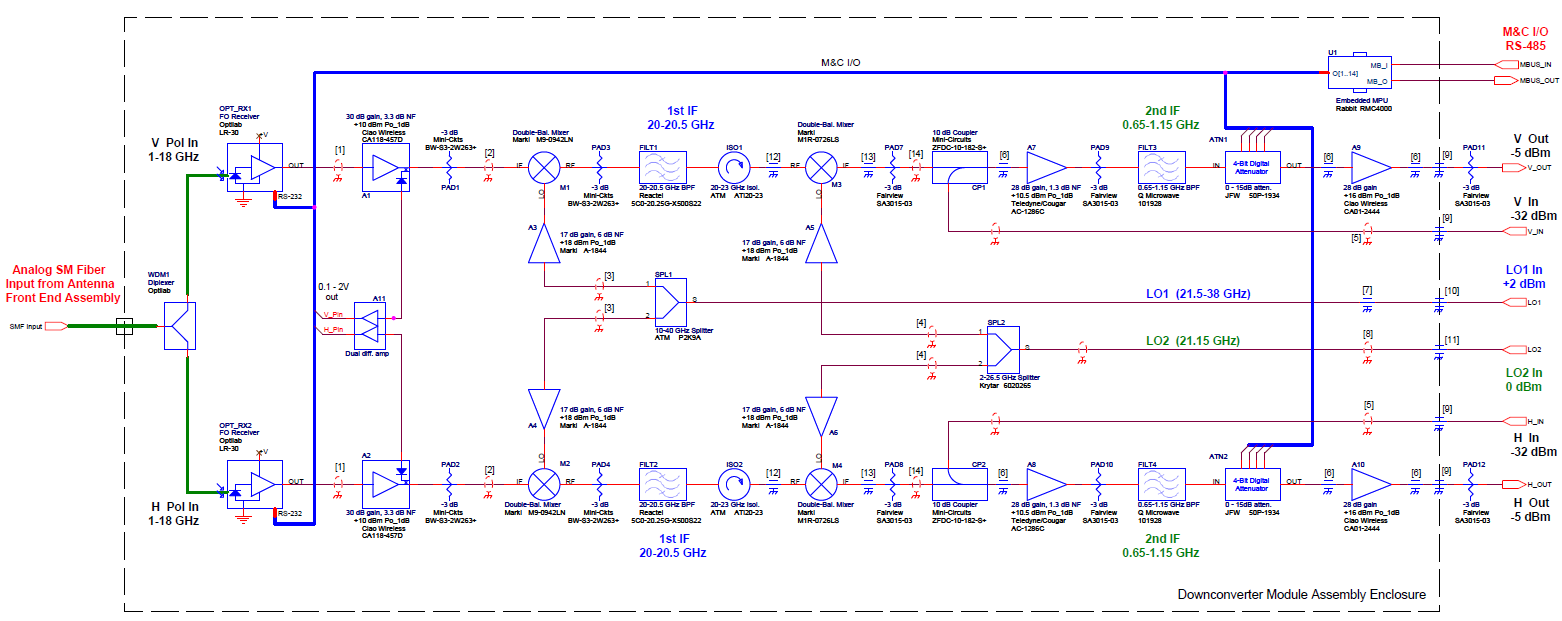
\includegraphics[scale=.25]{Figure_1.png}\footnotemark

\smallskip
The digital revolution has changed many aspects of modern life.  Scientific instrumentation has been no exception.  
\footnotetext[1]{$https://web.njit.edu/gary/728/assets/EOVSA\_DCM.PNG$}
\end{frame}

\begin{frame}
\frametitle{Et Tu, Science? The Fall Analog.}
In the EOVSA array, the signal is digitized at the receiver, then sent to the control room.  Why? 
\end{frame}

\begin{frame}
\frametitle{Digital vs. Analog: A Phase Fight}
In analog systems, the gain to phase balance of a signal cannot be maintained to better than $1\%$ over a range of temperatures (Harris, 2005).\footnotemark

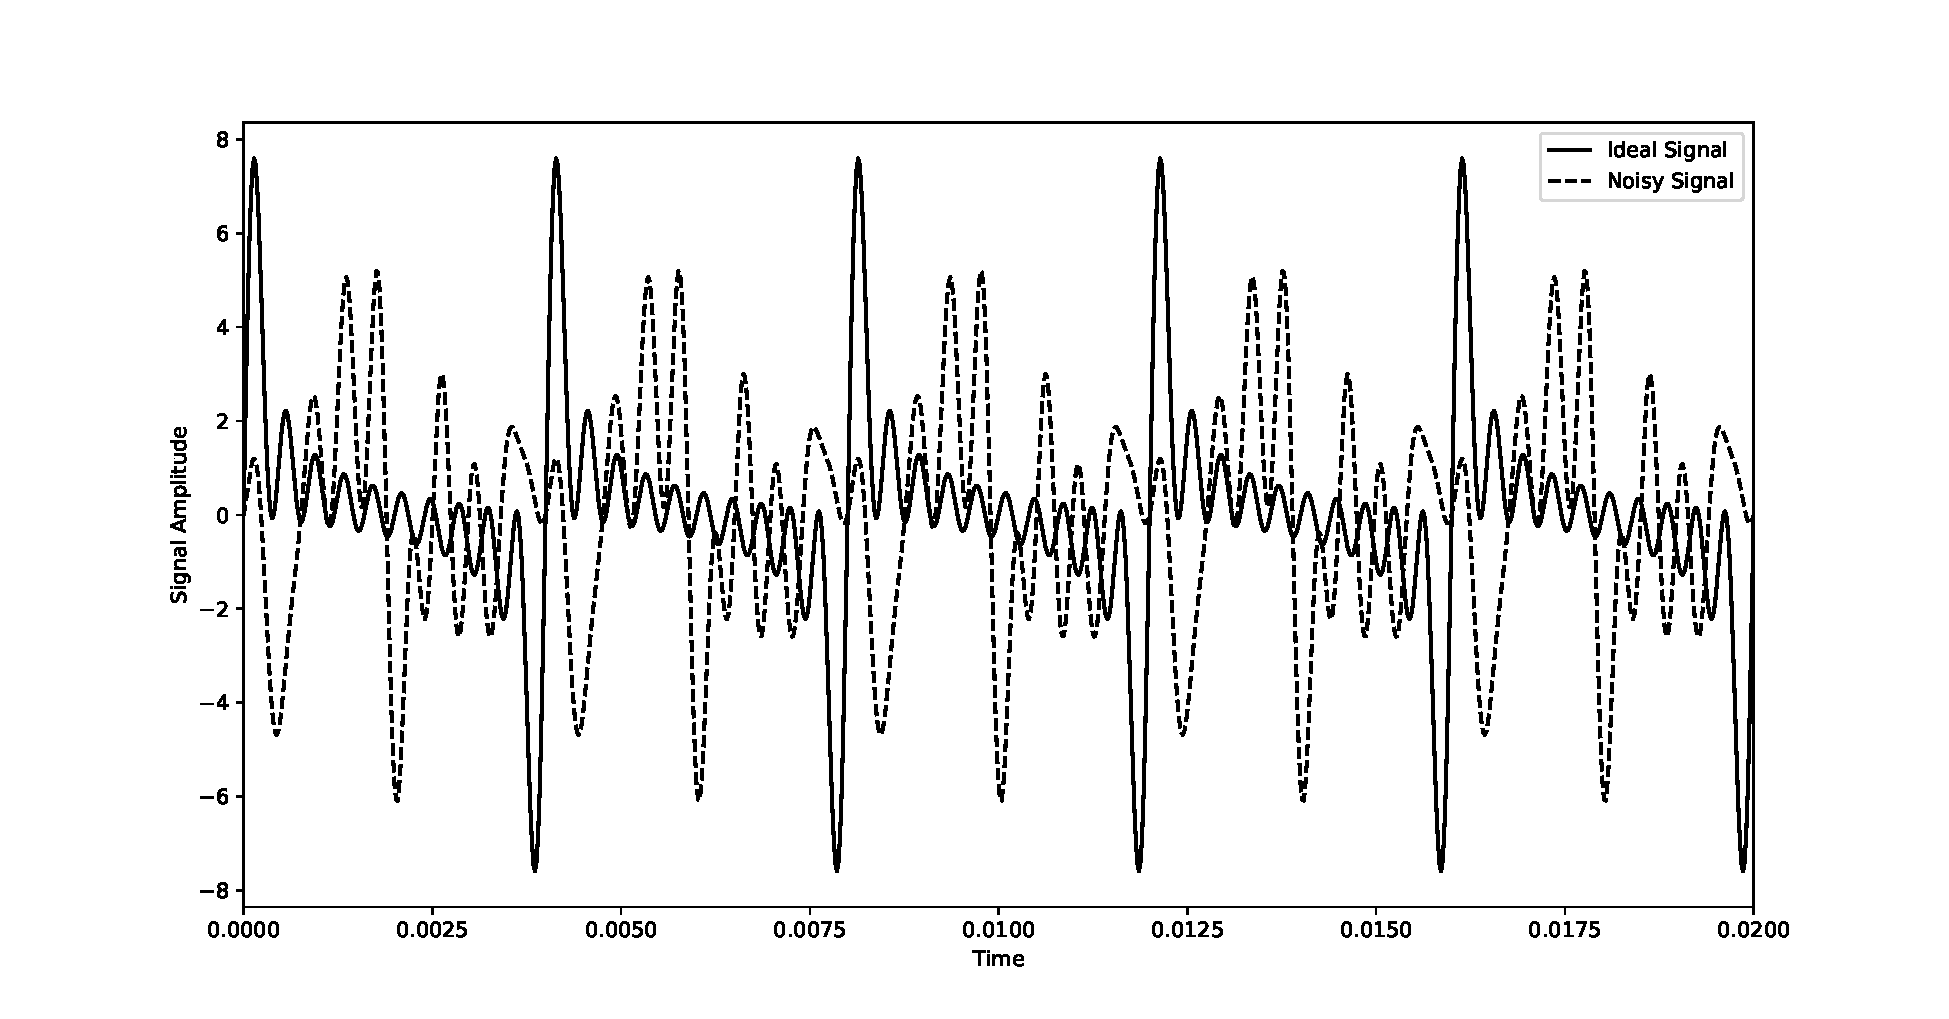
\includegraphics[scale=.35]{Figure_2.pdf}
\footnotetext[2]{Paper Citation}
\end{frame}

\begin{frame}
\frametitle{Signals, Nyquist Theorem, and Frequency Resolution}
\center \textbf{How do we digitize signals?}
\bigskip
\begin{columns}
\column{0.5\textwidth}
Nyquist Theorem
\begin{equation}
f_{crit} = \frac{f_{samp}}{2}
\end{equation}
In radio astronomy, to measure a 10 GHz signal, we would need to process 20 billion samples, or around 160 Gigabytes of data, a second.  Seem unreasonable? It is.
\column{0.5\textwidth}
Along with Nyquist, there is a limit to how much resolution there is between frequencies when using Fast Fourier Transform(FFT), which is given by 
\begin{equation}
f_{res} = f_{samp}/N
\end{equation}
where N is the number of sample points given to the FFT.
\end{columns}
\end{frame}

\begin{frame}
\frametitle{Downconversion:  The Hero Gotham Deserves}
\center Downconversion allows us to get around the absurd data requirement above. But how?
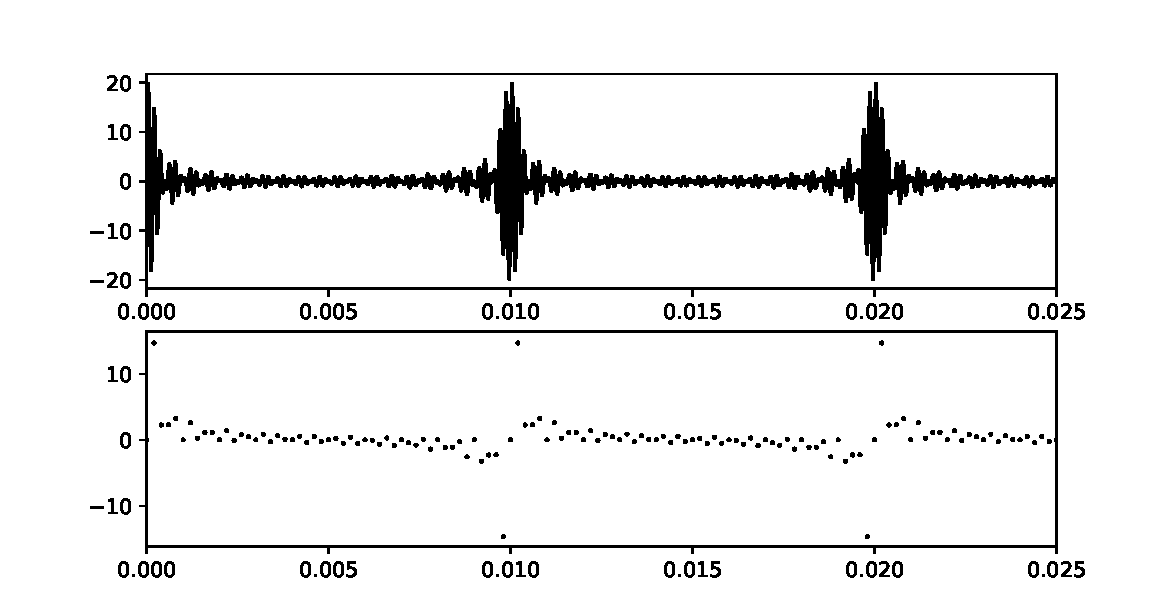
\includegraphics[scale=.5]{Figure_3.pdf}
\end{frame}

\begin{frame}
\frametitle{Downconversion:  The Hero Gotham Deserves}
This is a text in the first frame. This is a text in the first frame. This is a text in the first frame.
\end{frame}

\begin{frame}
\frametitle{Side Lobes: A Pain in the Power Spectra}
This is a text in the first frame. This is a text in the first frame. This is a text in the first frame.
\end{frame}

\begin{frame}
\frametitle{Side Lobes: A Pain in the Power Spectra}
This is a text in the first frame. This is a text in the first frame. This is a text in the first frame.
\end{frame}

\begin{frame}
\frametitle{Windowing Functions: The Good, the Bad, and the Unresolved}
This is a text in the first frame. This is a text in the first frame. This is a text in the first frame.
\end{frame}

\begin{frame}
\frametitle{Windowing Functions: The Good, the Bad, and the Unresolved}
This is a text in the first frame. This is a text in the first frame. This is a text in the first frame.
\end{frame}

\begin{frame}
\frametitle{Windowing Functions: The Good, the Bad, and the Unresolved}
This is a text in the first frame. This is a text in the first frame. This is a text in the first frame.
\end{frame}

\begin{frame}
\frametitle{Filter Banks}
This is a text in the first frame. This is a text in the first frame. This is a text in the first frame.
\end{frame}

\begin{frame}
\frametitle{The Polyphase Implementation: An Example}
This is a text in the first frame. This is a text in the first frame. This is a text in the first frame.
\end{frame}

\begin{frame}
\frametitle{The Polyphase Implementation: An Example}
This is a text in the first frame. This is a text in the first frame. This is a text in the first frame.
\end{frame}

\begin{frame}
\frametitle{The Polyphase Implementation: An Example}
This is a text in the first frame. This is a text in the first frame. This is a text in the first frame.
\end{frame}

\begin{frame}
\frametitle{When Windows Break: Channelizers and Polyphase Implementation}
This is a text in the first frame. This is a text in the first frame. This is a text in the first frame.
\end{frame}

\begin{frame}
\frametitle{Complicate the Theory, Simplify the Hardware?}
This is a text in the first frame. This is a text in the first frame. This is a text in the first frame.
\end{frame}

\begin{frame}
\frametitle{Complicate the Theory, Simplify the Hardware?}
This is a text in the first frame. This is a text in the first frame. This is a text in the first frame.
\end{frame}

\begin{frame}
\frametitle{The Universe Talks in Channels?}
This is a text in the first frame. This is a text in the first frame. This is a text in the first frame.
\end{frame}

\begin{frame}
\frametitle{The Universe Talks in Channels?}
This is a text in the first frame. This is a text in the first frame. This is a text in the first frame.
\end{frame}

\begin{frame}
\frametitle{The Universe Talks in Channels?}
This is a text in the first frame. This is a text in the first frame. This is a text in the first frame.
\end{frame}
\end{document}

